\section{Численные эксперименты: геометрия и возмущения}

В предыдущих разделах устойчивость и топология орбит исследовались с помощью матрицы монодромии и координатных преобразований. В этом разделе мы приводим прямые численные эксперименты, которые, во-первых, показывают, как орбиты выглядят в инерциальной (абсолютной) системе отсчёта, а во-вторых, подтверждают, что вычисленный показатель Ляпунова \(\lambda\) действительно предсказывает скорость расхождения траекторий при малых начальных возмущениях.

\subsection{Орбиты в инерциальной системе отсчёта: розетки}
Состояния в каталогах записаны во вращающейся системе отсчёта. Для перехода в инерциальную систему необходимо учесть поворот на угол \(\Omega t\) (а для блока \textit{unified} — ещё и снять начальный поворот \(-\theta\), применённый в каталоге).

Если интегрировать орбиту в инерциальной системе ровно на один период \(T\), то траектория не замыкается: рамка вращается, и за период накапливается поворот на угол \(\Delta\varphi = \Omega T\). Для орбит блока \textit{arclength} отношение \(\Omega T / (2\pi) \approx 1.2452 \approx 5/4\), то есть за один период рамка делает \(1\frac{1}{4}\) оборота. Поэтому, чтобы получить замкнутую «розетку», необходимо собрать \(K\) копий одной и той же проинтегрированной траектории, каждая из которых повёрнута на угол \(k \cdot \Omega T\) (\(k = 0, \dots, K-1\)). Для \(5/4\) достаточно \(K=4\): накопленный поворот составит \(5\) полных оборотов, и роза замкнётся с точностью до \(0.4\%\). Такой подход позволяет избежать накопления ошибок интегрирования на длинных временах (что критично для неустойчивых орбит).

Для орбит блока \textit{canonical} отношение \(\Omega T / (2\pi) \approx 0.61\), поэтому «розетки» там нет — тела движутся по почти круговым орбитам, и достаточно интегрировать один оборот барицентра \(T_{rot} = 2\pi/\Omega\) с \(K=1\).

Результаты для нескольких репрезентативных орбит показаны на рисунке~\ref{fig:inertial_grid}. Видно, что орбиты блока \textit{arclength} (нижние панели) образуют характерные 5-лепестковые розетки, а орбиты \textit{canonical} (верхние панели) — почти круговые.

\begin{figure}[H]
    \centering
    \includegraphics[width=\textwidth]{93_inertial_grid_v4.png}
    \caption{Орбиты в инерциальной системе отсчёта. Верхний ряд: блок \textit{canonical} (интегрирование одного оборота барицентра, \(K=1\)). Нижние ряды: блок \textit{arclength} (сборка из \(K=4\) копий одного периода, 5-лепестковые розетки).}
    \label{fig:inertial_grid}
\end{figure}

Отдельно на рисунке~\ref{fig:U5000_unstable} показано, как выглядит неустойчивая орбита \(U\,5000\) (блок \textit{canonical}, \(\max|\mu| \approx 826\)) при интегрировании на 1, 2 и 3 периода. Уже на втором периоде видно, что тело 2 уходит из центра, а тела 1 и 3 сходят со своих почти круговых орбит — это прямое визуальное проявление неустойчивости.

\begin{figure}[H]
    \centering
    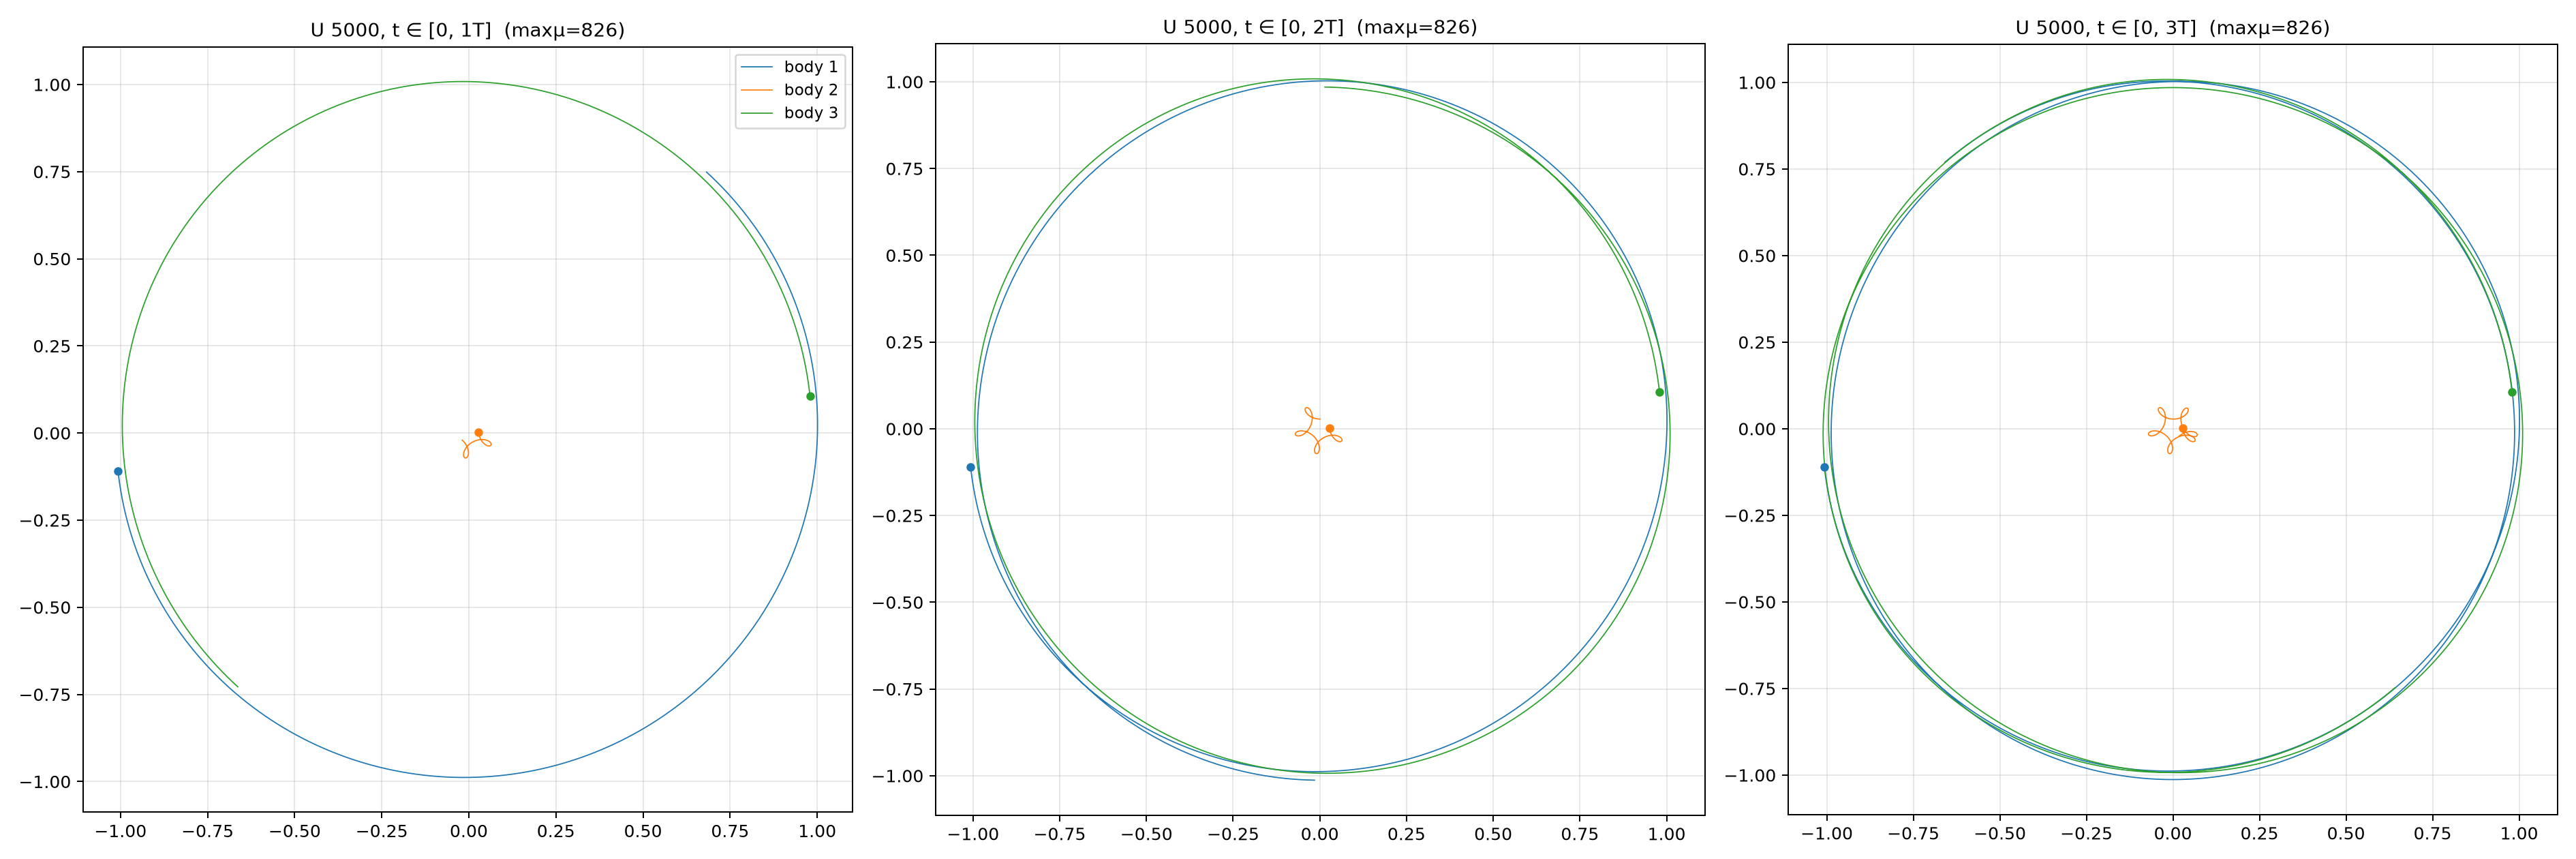
\includegraphics[width=\textwidth]{93d_U5000_1T_2T_3T.png}
    \caption{Неустойчивая орбита \(U\,5000\) в инерциальной системе при интегрировании на 1, 2 и 3 периода. Видно, как на втором периоде траектории начинают «разваливаться» из-за неустойчивости.}
    \label{fig:U5000_unstable}
\end{figure}

\subsection{Тесты на возмущение: рост \(| \Delta X(t) |\)}
Для прямой проверки связи между мультипликаторами Флоке и реальной скоростью расхождения траекторий был проведён следующий эксперимент. Берётся начальное состояние \(X_0\) из каталога и возмущённое состояние \(X_0 + \delta X\), где возмущение вносится только в координату \(y_1\): \(\delta y_1 = \delta\). Обе орбиты интегрируются на \(K\) периодов, и вычисляется евклидово расстояние в 8-мерном фазовом пространстве:
\begin{equation}
    |\Delta X(t)| = \| X(t; X_0) - X(t; X_0 + \delta X) \|.
\end{equation}
Согласно линейной теории, при малых \(\delta\) это расстояние должно расти как
\begin{equation}
    |\Delta X(t)| \approx C \cdot \delta \cdot e^{\lambda t}, \quad \lambda = \frac{\ln(\max|\mu|)}{T}.
\end{equation}
Коэффициент \(C\) зависит от того, насколько начальное возмущение \(\delta X\) «выровнено» по неустойчивому собственному вектору матрицы монодромии.

На рисунке~\ref{fig:pert_A1593} показаны результаты для орбиты \(A\,1593\) (блок \textit{arclength}). Слева — орбиты во вращающейся системе (исходная и возмущённая), в центре — \(| \Delta X(t) |\), справа — значения \(| \Delta X(nT) |\) в концах периодов и линейный фит. Видно, что \(\lambda_{\text{fit}} \approx 0.319\) практически совпадает с каталожным \(\lambda_{\text{cat}} \approx 0.324\). Это подтверждает, что вычисленный из матрицы монодромии показатель Ляпунова правильно предсказывает скорость расхождения траекторий.

\begin{figure}[H]
    \centering
    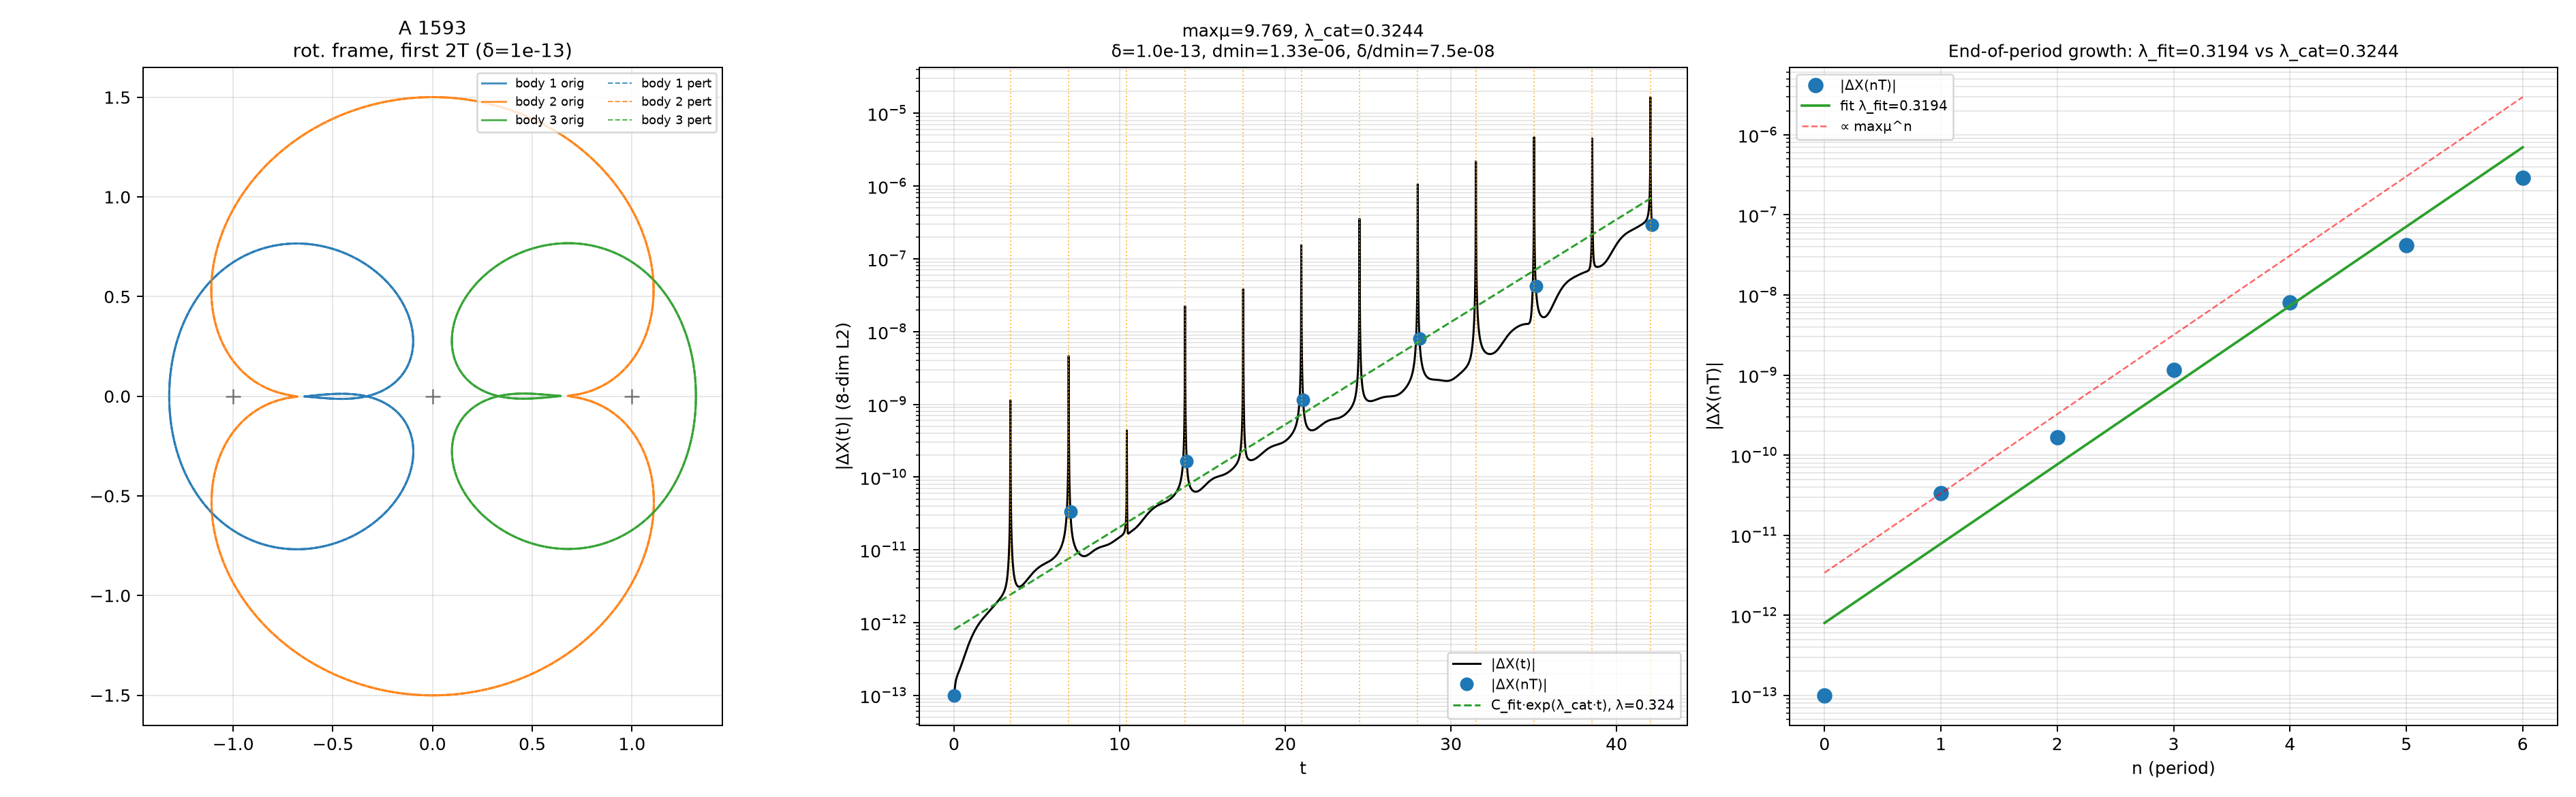
\includegraphics[width=\textwidth]{93_pert_A_1593.png}
    \caption{Тест на возмущение для орбиты \(A\,1593\) (\(\delta=10^{-13}\), \(K=6\)). Слева: орбиты во вращающейся системе (первые 2 периода). В центре: \(| \Delta X(t) |\). Справа: \(| \Delta X(nT) |\) и линейный фит \(\lambda_{\text{fit}} \approx 0.319\) (каталожное \(\lambda_{\text{cat}} \approx 0.324\)).}
    \label{fig:pert_A1593}
\end{figure}

Аналогичные результаты получены для орбиты \(A\,1641\) (рисунок~\ref{fig:pert_A1641}), где \(\lambda_{\text{fit}} \approx 0.381\) против \(\lambda_{\text{cat}} \approx 0.325\). Небольшое превышение объясняется нелинейными эффектами в моменты сближений (пики на центральной панели), но общий экспоненциальный закон выполняется.

\begin{figure}[H]
    \centering
    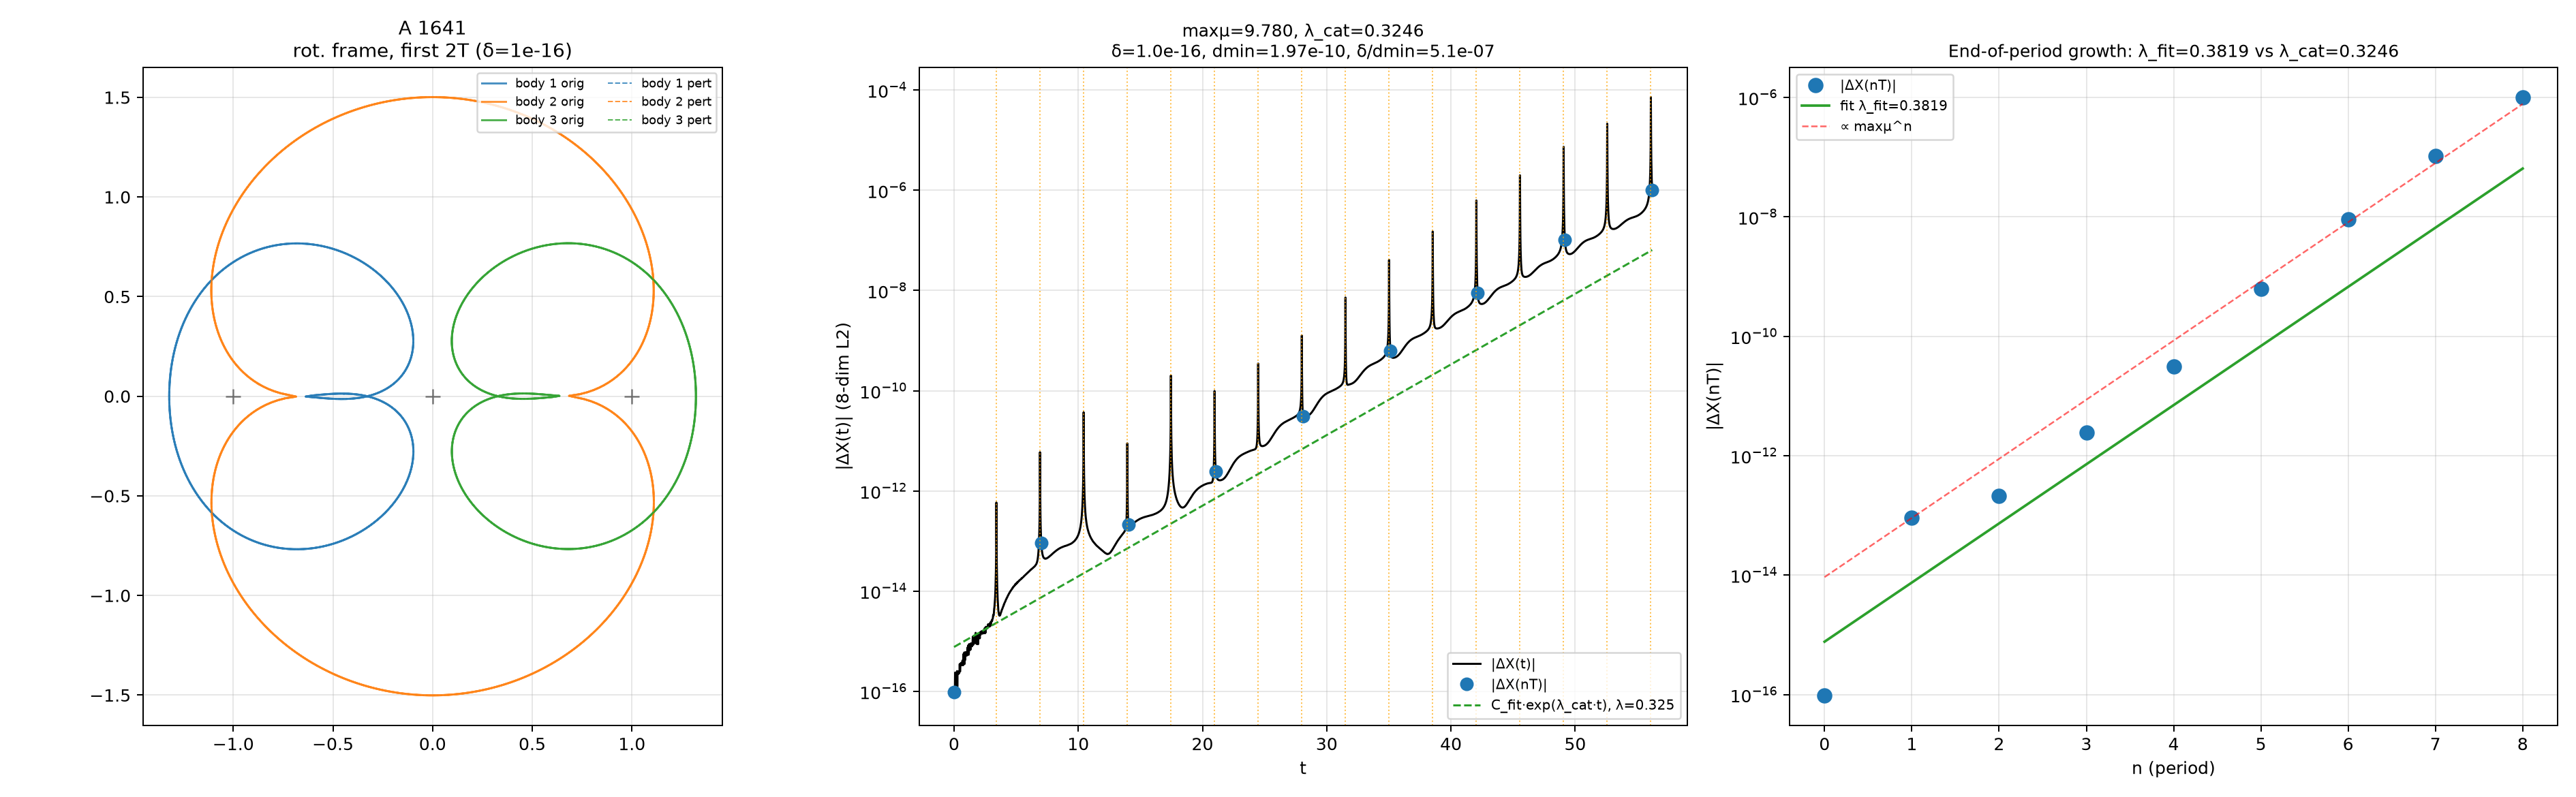
\includegraphics[width=\textwidth]{93_pert_A_1641.png}
    \caption{Тест на возмущение для орбиты \(A\,1641\) (\(\delta=10^{-16}\), \(K=8\)). \(\lambda_{\text{fit}} \approx 0.381\) против \(\lambda_{\text{cat}} \approx 0.325\).}
    \label{fig:pert_A1641}
\end{figure}

\subsection{Нелинейное насыщение на примере \(U\,5000\)}
Для сильно неустойчивой орбиты \(U\,5000\) (\(\max|\mu| \approx 826\), \(\lambda \approx 1.94\)) тест на возмущение демонстрирует важный нелинейный эффект: насыщение. При \(\delta = 10^{-7}\) возмущение растёт экспоненциально только до \(t \approx 9\), после чего \(| \Delta X(t) |\) выходит на плато \(\sim 10\) (рисунок~\ref{fig:pert_U5000}). Это происходит потому, что расстояние между двумя траекториями достигает размера всей фазовой области, и линейная теория перестаёт работать.

\begin{figure}[H]
    \centering
    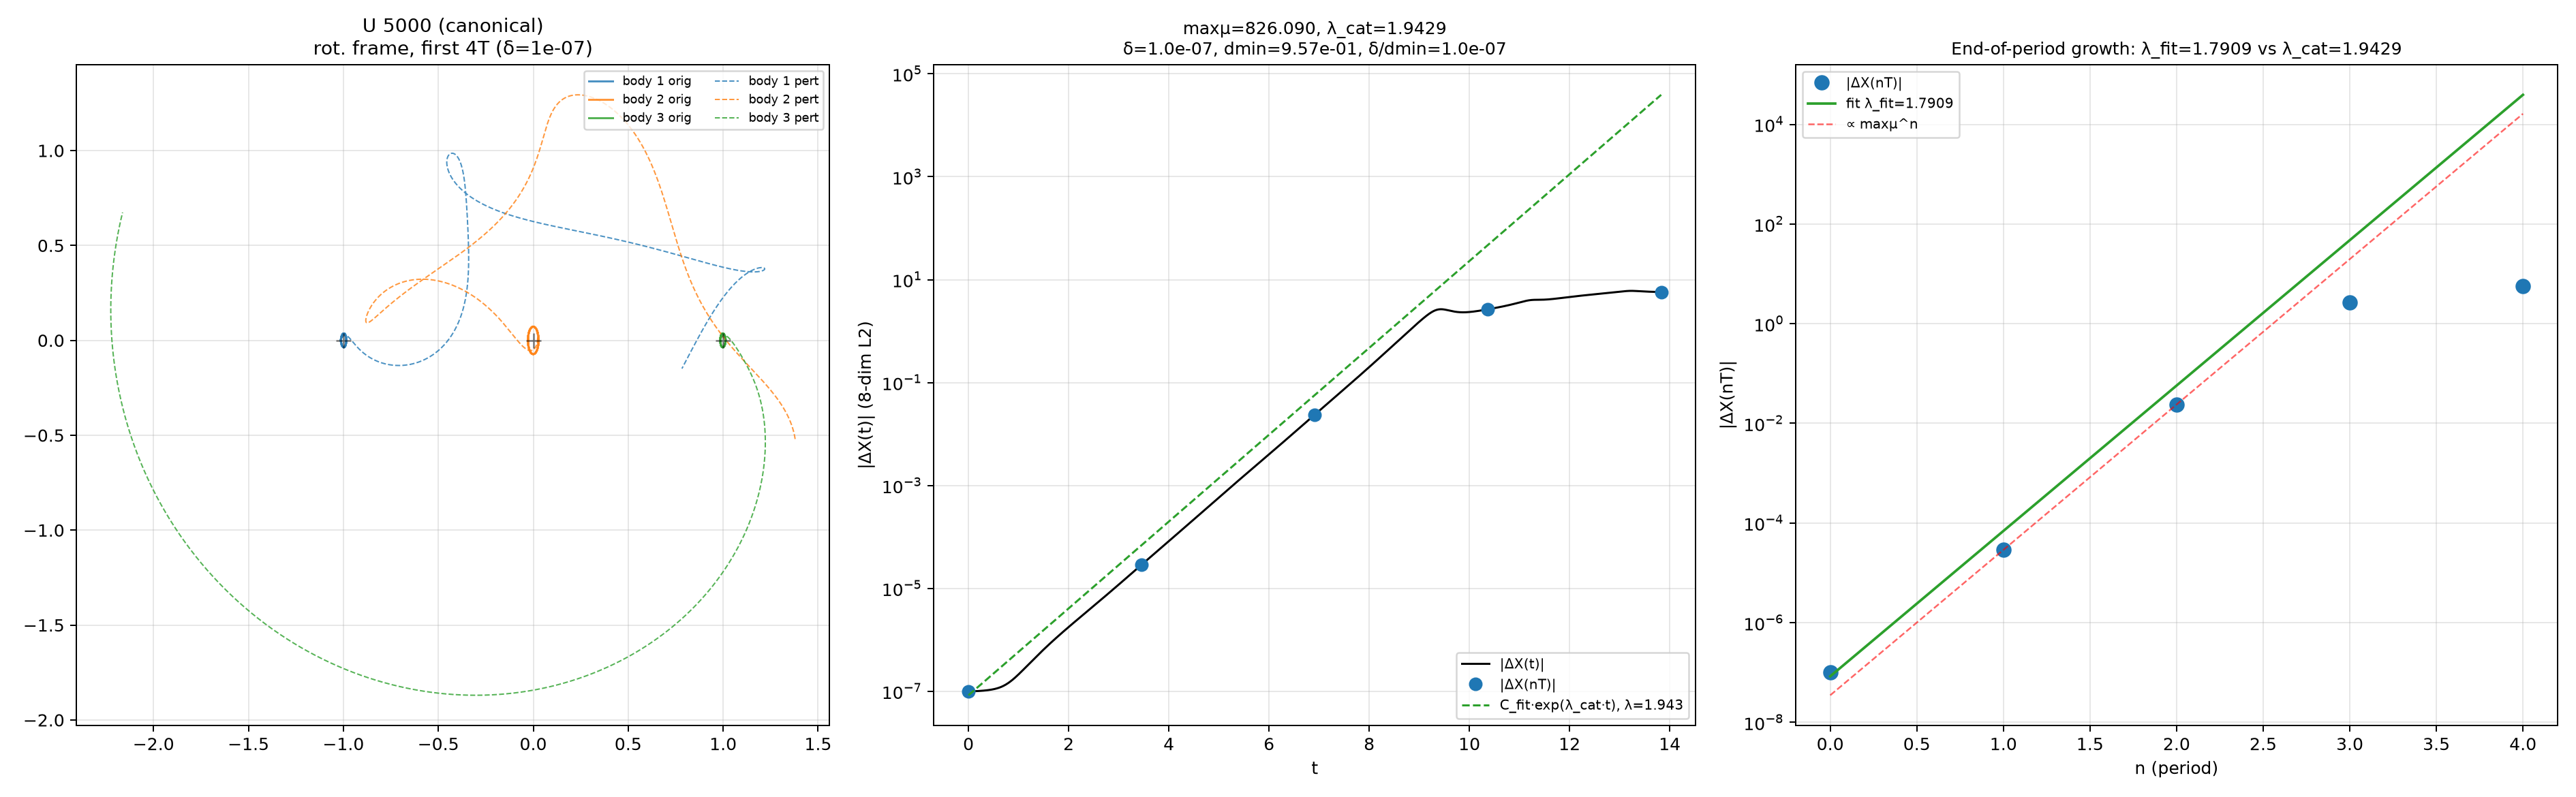
\includegraphics[width=\textwidth]{93_pert_U_5000.png}
    \caption{Тест на возмущение для орбиты \(U\,5000\) (\(\delta=10^{-7}\), \(K=4\)). Виден экспоненциальный рост \(| \Delta X(t) |\) до \(t \approx 9\) и последующее насыщение.}
    \label{fig:pert_U5000}
\end{figure}

Из-за насыщения линейный фит по всем 4 периодам даёт заниженное значение \(\lambda_{\text{fit}} \approx 1.79\) вместо \(\lambda_{\text{cat}} \approx 1.94\). Если же использовать только первые 2–3 периода (до насыщения), фит совпадает с теоретическим значением. Этот пример наглядно показывает границы применимости линейного анализа.

\subsection{Вывод по численным экспериментам}
Проведённые тесты подтверждают:
\begin{enumerate}
    \item Показатель Ляпунова \(\lambda = \ln(\max|\mu|)/T\), вычисленный из матрицы монодромии, правильно предсказывает скорость расхождения траекторий при малых возмущениях (для линейного режима \(\lambda_{\text{fit}} \approx \lambda_{\text{cat}}\)).
    \item На больших временах или при больших \(\delta\) проявляются нелинейные эффекты (насыщение), которые ограничивают применимость линейной теории.
    \item В инерциальной системе орбиты блока \textit{arclength} образуют 5-лепестковые розетки, что является геометрическим следствием отношения \(\Omega T/(2\pi) \approx 5/4\), а не резонансным захватом.
\end{enumerate}